% 	Name		:: 	sthlm Beamer Theme  HEAVILY based on the hsrmbeamer theme (Benjamin Weiss)
%	Author		:: 	Mark Hendry Olson (mark@hendryolson.com)
%	Created		::	2013-07-31
%	Updated		::	June 18, 2015 at 08:45
%	Version		:: 	1.0.2
%	Email		:: 	hendryolson@gmail.com
%	Website		:: 	http://v42.com
%
% 	License		:: 	This file may be distributed and/or modified under the
%                  	GNU Public License.
%
%	Description	::	This presentation is a demonstration of the sthlm beamer
%					theme, which is HEAVILY based on the HSRM beamer theme created by Benjamin Weiss
%					(benjamin.weiss@student.hs-rm.de), which can be found on GitHub
%					<https://github.com/hsrmbeamertheme/hsrmbeamertheme>.


%-=-=-=-=-=-=-=-=-=-=-=-=-=-=-=-=-=-=-=-=-=-=-=-=
%
%        LOADING DOCUMENT
%
%-=-=-=-=-=-=-=-=-=-=-=-=-=-=-=-=-=-=-=-=-=-=-=-=

\documentclass[newPxFont]{beamer}
\usetheme{sthlm}
%\usecolortheme{sthlmv42}

%-=-=-=-=-=-=-=-=-=-=-=-=-=-=-=-=-=-=-=-=-=-=-=-=
%        LOADING PACKAGES
%-=-=-=-=-=-=-=-=-=-=-=-=-=-=-=-=-=-=-=-=-=-=-=-=
\usepackage[utf8]{inputenc}
\usepackage[T1]{fontenc}

%\usepackage{chronology}
\usepackage{chronosys}
\usepackage{subfigure}

\newcommand{\tabitem}{%
  \usebeamertemplate{itemize item}\hspace*{\labelsep}}

%\renewcommand{\event}[3][e]{%
%  \pgfmathsetlength\xstop{(#2-\theyearstart)*\unit}%
%  \ifx #1e%
%    \draw[fill=black,draw=none,opacity=0.5]%
%      (\xstop, 0) circle (.2\unit)%
%      node[opacity=1,rotate=45,right=.2\unit] {#3};%
%  \else%
%    \pgfmathsetlength\xstart{(#1-\theyearstart)*\unit}%
%    \draw[fill=black,draw=none,opacity=0.5,rounded corners=.1\unit]%
%      (\xstart,-.1\unit) rectangle%
%      node[opacity=1,rotate=45,right=.2\unit] {#3} (\xstop,.1\unit);%
%  \fi}%

%-=-=-=-=-=-=-=-=-=-=-=-=-=-=-=-=-=-=-=-=-=-=-=-=
%        BEAMER OPTIONS
%-=-=-=-=-=-=-=-=-=-=-=-=-=-=-=-=-=-=-=-=-=-=-=-=

%\setbeameroption{show notes}

%-=-=-=-=-=-=-=-=-=-=-=-=-=-=-=-=-=-=-=-=-=-=-=-=
%
%	PRESENTATION INFORMATION
%
%-=-=-=-=-=-=-=-=-=-=-=-=-=-=-=-=-=-=-=-=-=-=-=-=

\title{A Great Green Wall social-ecological systems database}
\subtitle{A tool for researchers and managers}
%\date{\small{\jobname}}
%\date{\today}
\date{15 juin 2016}
\author{\texttt{ E. Delay}}
\institute{\textsc{Ohm} Téssékéré - Sénégal}

\hypersetup{
pdfauthor = {E. DELAY},
pdfsubject = {Réseau OHM},
pdfkeywords = {grande muraille verte, ANR future Sahel},
pdfmoddate= {D:\pdfdate},
pdfcreator = {}
}

\begin{document}

%-=-=-=-=-=-=-=-=-=-=-=-=-=-=-=-=-=-=-=-=-=-=-=-=
%
%	TITLE PAGE
%
%-=-=-=-=-=-=-=-=-=-=-=-=-=-=-=-=-=-=-=-=-=-=-=-=

\maketitle

%\begin{frame}[plain]
%	\titlepage
%\end{frame}

%-=-=-=-=-=-=-=-=-=-=-=-=-=-=-=-=-=-=-=-=-=-=-=-=
%
%	TABLE OF CONTENTS: OVERVIEW
%
%-=-=-=-=-=-=-=-=-=-=-=-=-=-=-=-=-=-=-=-=-=-=-=-=
%\section*{Overview}
%\begin{frame}{Overview}
%% For longer presentations use hideallsubsections option
%\tableofcontents[hideallsubsections]
%\end{frame}

%-=-=-=-=-=-=-=-=-=-=-=-=-=-=-=-=-=-=-=-=-=-=-=-=
%	FRAME: INTRODUCTION
%-=-=-=-=-=-=-=-=-=-=-=-=-=-=-=-=-=-=-=-=-=-=-=-=

\section{Introduction}

%-=-=-=-=-=-=-=-=-=-=-=-=-=-=-=-=-=-=-=-=-=-=-=-=
%	FRAME: ANR framework in 4 wp
%-=-=-=-=-=-=-=-=-=-=-=-=-=-=-=-=-=-=-=-=-=-=-=-=
\begin{frame}[c]{The Great Green Wall}
\vspace{-1cm}
Yes, the Green Great Wall can be in China, by our sandbox is in Africa, where we work for the "Future Sahel" ANR project.
\begin{figure}
	\centering
	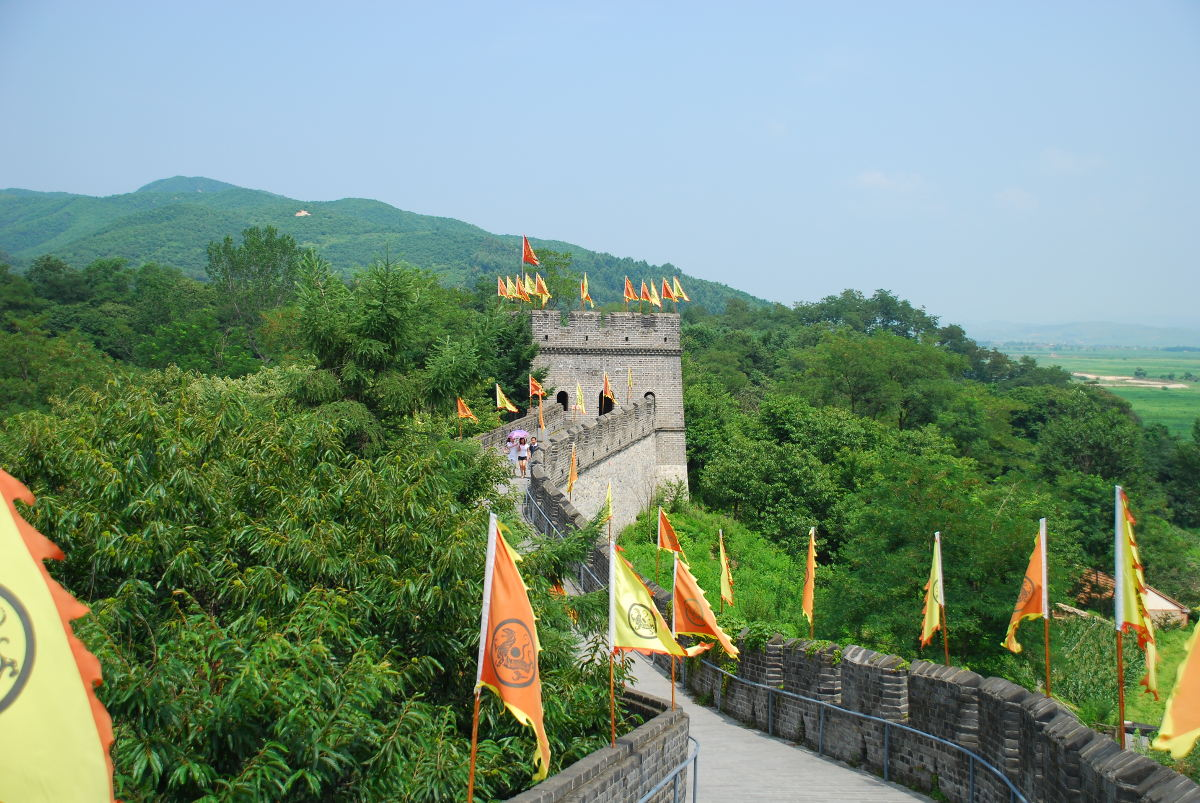
\includegraphics[width = 0.6\textwidth]{img/great_wall}
\end{figure}
\begin{center}
    \begin{tabular}{@{}l@{}}
       \\
      \tabitem width $\approx 15 km$ \\
      \tabitem length $\approx 7600km$
  \end{tabular}
\end{center}
\end{frame}

%-=-=-=-=-=-=-=-=-=-=-=-=-=-=-=-=-=-=-=-=-=-=-=-=
%	FRAME: ANR framework in 4 wp
%-=-=-=-=-=-=-=-=-=-=-=-=-=-=-=-=-=-=-=-=-=-=-=-=
\begin{frame}[c]{Future Sahel Framework}
\vspace{-1cm}
\begin{figure}
	\centering
	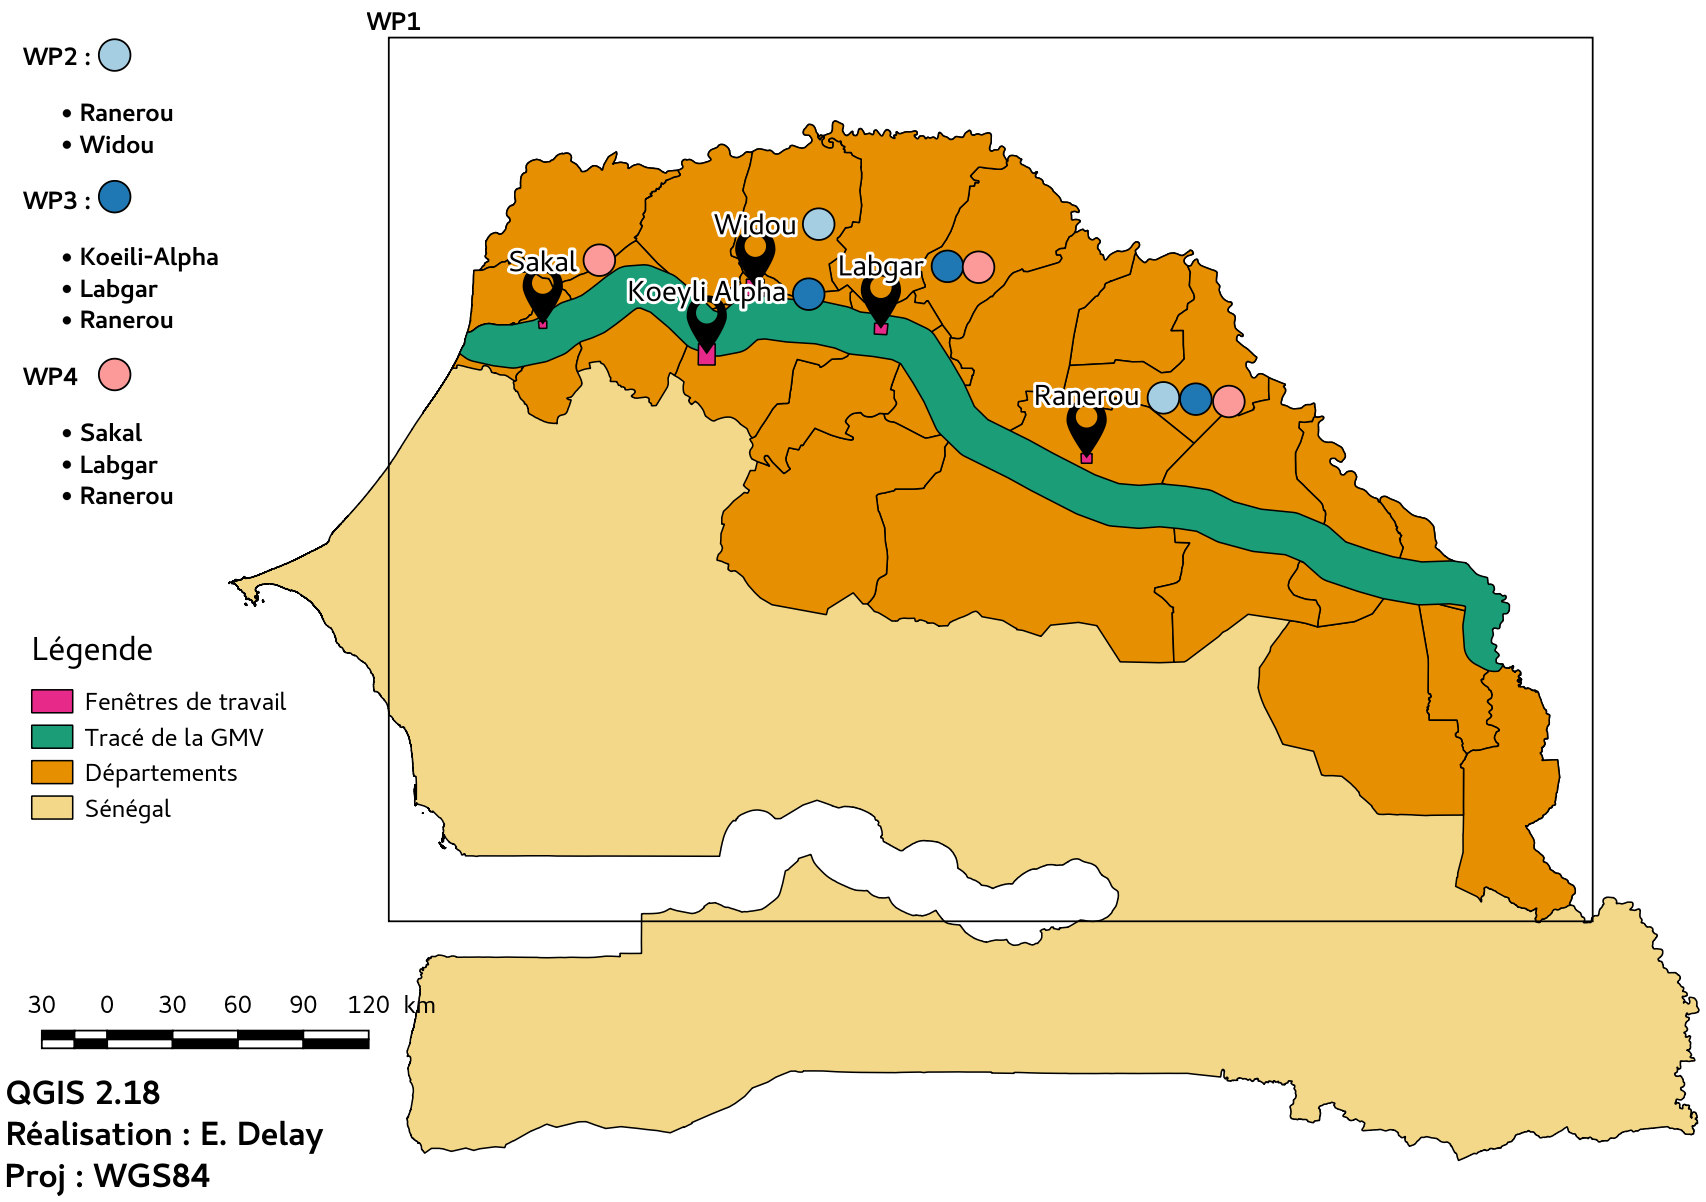
\includegraphics[width = 0.8\textwidth]{img/Carte_FutureSahel}
	\caption{FutureSahel Work Packages}
\end{figure}
\end{frame}

%-=-=-=-=-=-=-=-=-=-=-=-=-=-=-=-=-=-=-=-=-=-=-=-=
%	FRAME: ANR framework in 4 wp
%-=-=-=-=-=-=-=-=-=-=-=-=-=-=-=-=-=-=-=-=-=-=-=-=

\begin{frame}[c]{Focus on WP1}
\vspace{-1cm}
In close cooperation with the Senegalese agency of Green Great Wall (ANGMV), build a database for researcher and green great wall managers :
	\begin{itemize}
		\item researchers $\rightarrow$ maintain and exploit data produced in a research context (landscape ecology);
		\item managers $\rightarrow$ use knowledge for spatio-temporal planification.
	\end{itemize}
  \begin{figure}
  	\centering
  	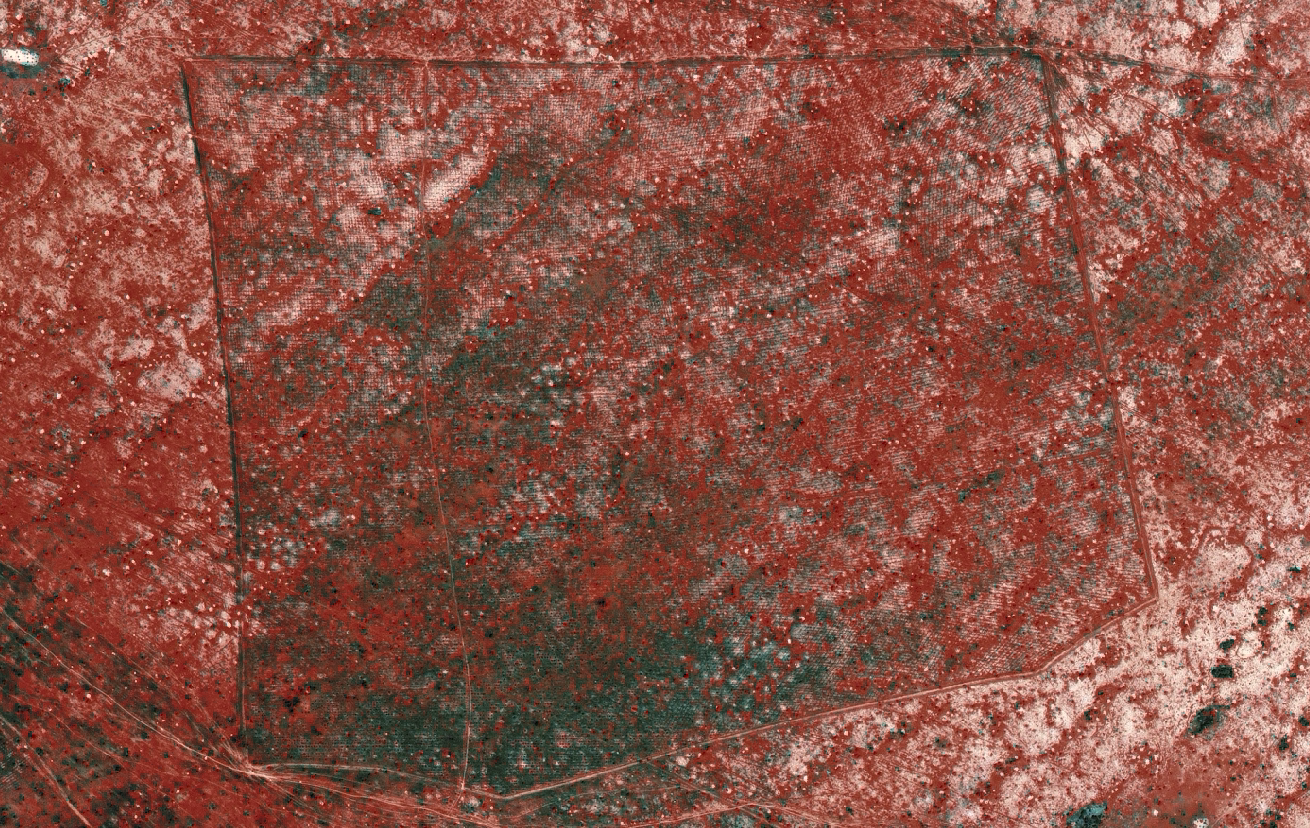
\includegraphics[width = 6cm]{img/IR_spot}
  \end{figure}
\end{frame}

%-=-=-=-=-=-=-=-=-=-=-=-=-=-=-=-=-=-=-=-=-=-=-=-=
%	FRAME: Goals for our SGBD
%-=-=-=-=-=-=-=-=-=-=-=-=-=-=-=-=-=-=-=-=-=-=-=-=

\begin{frame}[c]{Material and methods}
\vspace{-1cm}
\begin{itemize}
	\item The initial architecture developed on PostgreSQL and PostGIS (GEOLAB);
	\item Stay compatible with BBees metadata;
	\item We need to find a way to deal with heterogen space and time data :
	\begin{itemize}
		\item Raster (Spot, Modis, Landsat, Sentinel);
		\item statistical information produced by institutions;
		\item field data.
	\end{itemize}
	\item Technology transfer to stockholders (ANGMV), we need to choose free and open source software.
\end{itemize}
\begin{figure}
	\centering
	
\includegraphics[height=20mm]{img/PostGIS_logo}
	
\includegraphics[height=20mm]{img/QGis_Logo}
	
\includegraphics[height=20mm]{img/GrassGIS_banner}
	
\includegraphics[height=20mm]{img/Rlogo}
\end{figure}
\end{frame}

%-=-=-=-=-=-=-=-=-=-=-=-=-=-=-=-=-=-=-=-=-=-=-=-=
%	FRAME: context
%-=-=-=-=-=-=-=-=-=-=-=-=-=-=-=-=-=-=-=-=-=-=-=-=

\section{Pathway}

%-=-=-=-=-=-=-=-=-=-=-=-=-=-=-=-=-=-=-=-=-=-=-=-=
%	FRAME: WP
%-=-=-=-=-=-=-=-=-=-=-=-=-=-=-=-=-=-=-=-=-=-=-=-=

\begin{frame}[c]{WP1 : large-scale data}
\vspace{-2em}
Find data using the Institutional analysis and development (IDA) framework (Ostrom 2009)
\vspace{-1em}
\begin{figure}
	\centering
	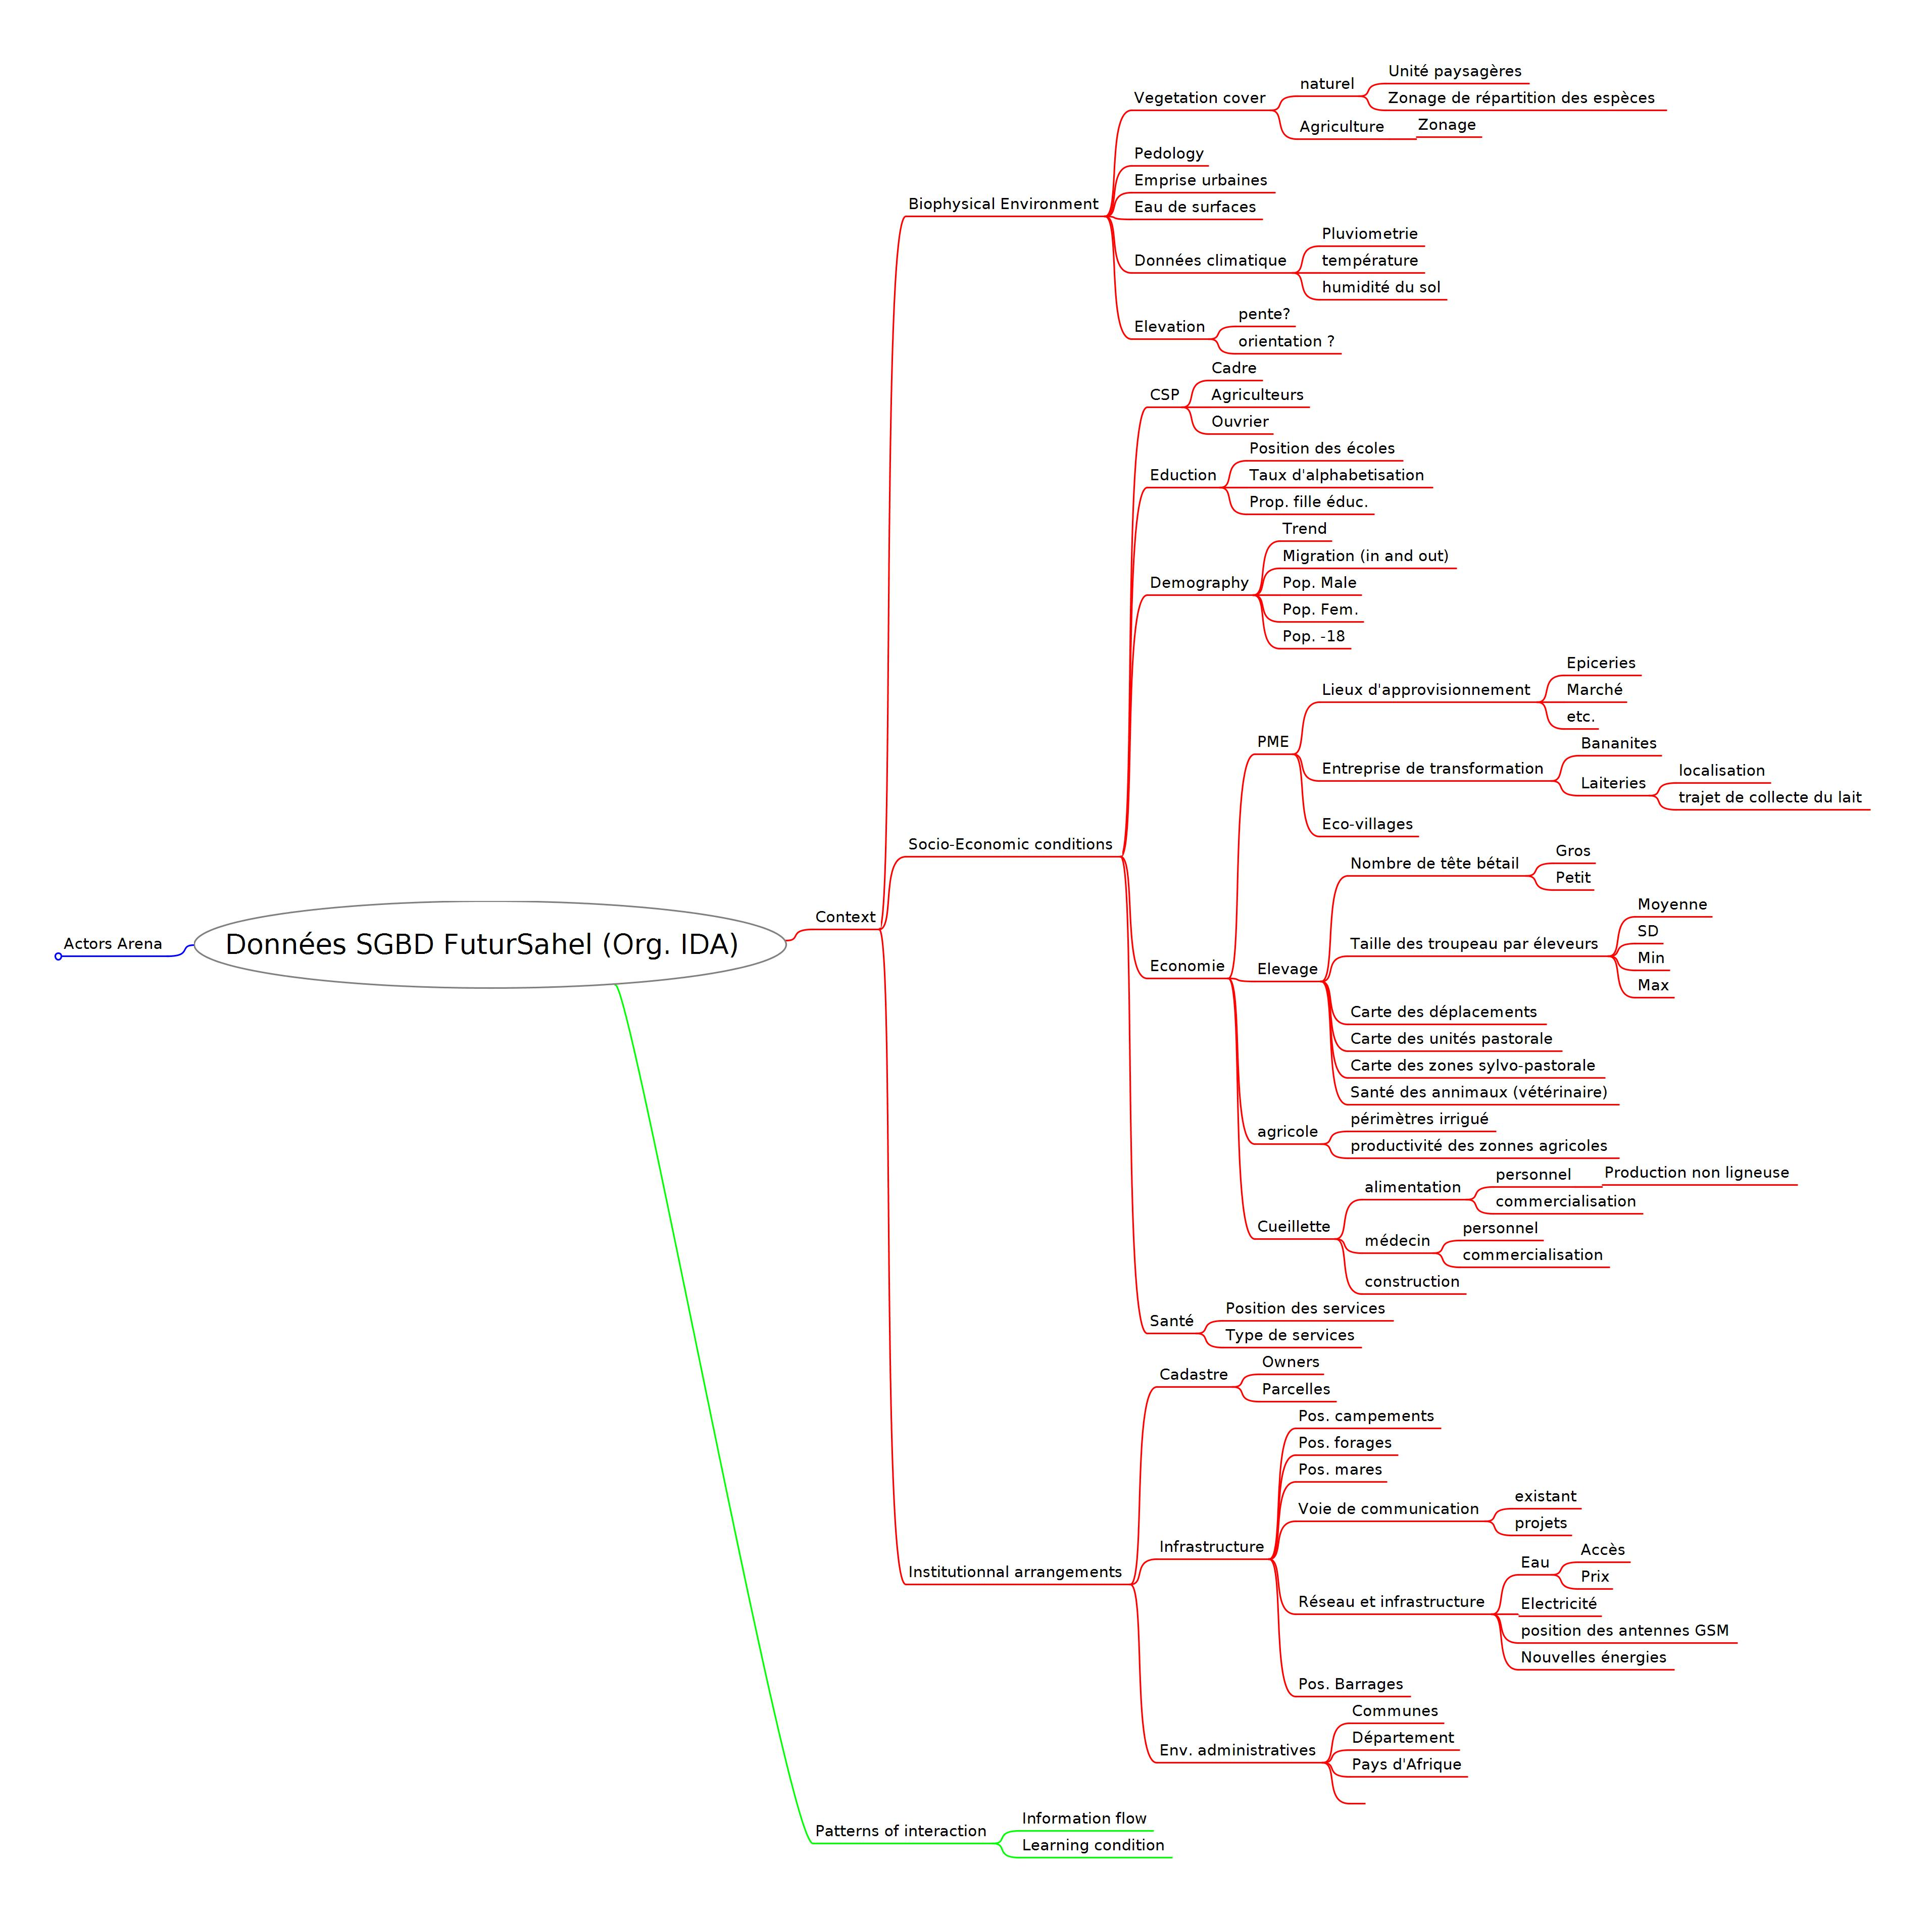
\includegraphics[width = 7cm]{img/IDA_data_org}
\end{figure}
\end{frame}

\begin{frame}[c]{WP1 : biophysical environment data}
\vspace{-2em}
\begin{itemize}
  \item Work in small windows
  \begin{itemize}
    \item Spot 6 images (1.5 m) $\rightarrow$ canopy, pond detection and NDVI calculation
    \item MODIS (250 m) $\rightarrow$ evaluation of tree NDVI participation
    \item Spot / Modis $\rightarrow$ evaluation of sahel greening?
  \end{itemize}
  \item Generalization $\rightarrow$ Sentinel ?
\end{itemize}
\vspace{-1em}
\begin{figure}
	\centering
	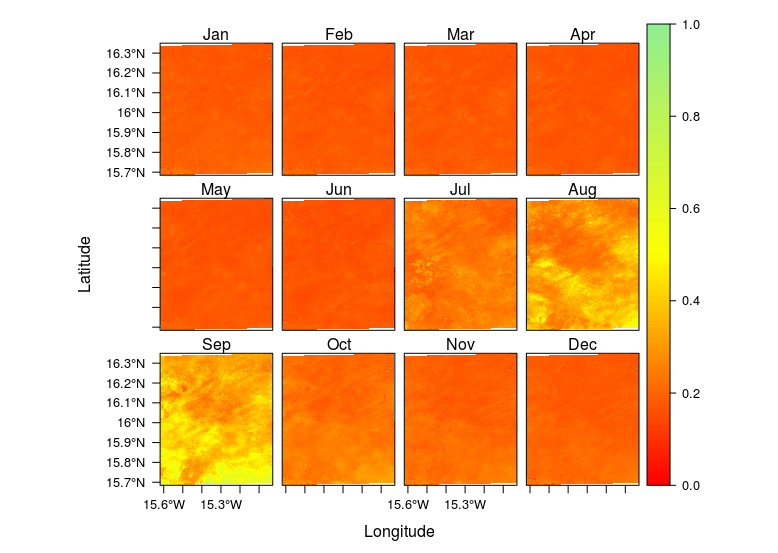
\includegraphics[width = 7cm]{img/NDVI2015}
\end{figure}
\end{frame}

%-=-=-=-=-=-=-=-=-=-=-=-=-=-=-=-=-=-=-=-=-=-=-=-=
%	FRAME: WP
%-=-=-=-=-=-=-=-=-=-=-=-=-=-=-=-=-=-=-=-=-=-=-=-=

\begin{frame}[c]{WP2 : plant biodiversity}
\vspace{-2em}
Maximize the plant biodiversity used in the GGW reforestation protocols. Initially, plantations were not very diversified, mainly composed of three species of trees: \textit{Balanites aegyptiaca}, \textit{Acacia senegal}, and \textit{Acacia tortilis subsp raddiana}.
\begin{itemize}
  \item new planting plots with other plan trees,
  \item \textit{in situ} ecological monitoring of planting trials.
\end{itemize}
\begin{figure}
	\centering
	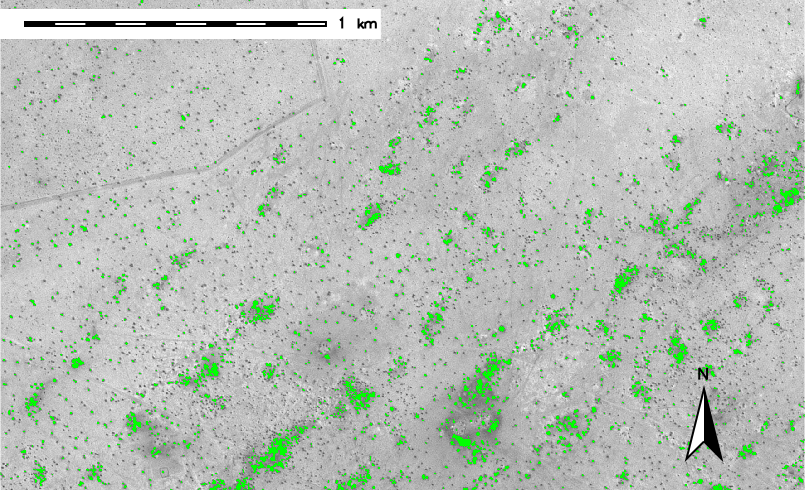
\includegraphics[width = 6cm]{img/Trees_sup15m2}
  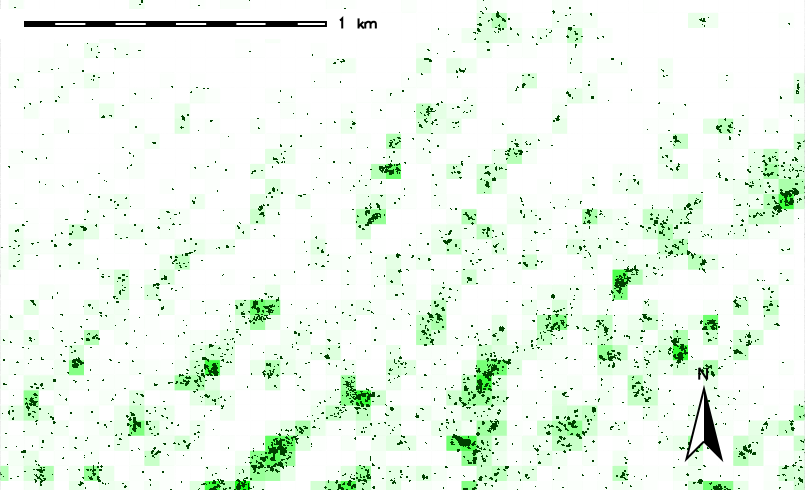
\includegraphics[width = 6cm]{img/GRID_Trees_sup15m2}
\end{figure}
\end{frame}
%-=-=-=-=-=-=-=-=-=-=-=-=-=-=-=-=-=-=-=-=-=-=-=-=
%	FRAME: WP
%-=-=-=-=-=-=-=-=-=-=-=-=-=-=-=-=-=-=-=-=-=-=-=-=

\begin{frame}[c]{WP3 : valorization of \textit{B. aegyptiaca} sector}
\vspace{-2em}
This species is widely used for various purposes by local populations  : fruts, oil extracted from the almond (cooking and cosmetics).
\begin{itemize}
  \item Biogeographic study,
  \item phenology and production (biomass, fruts),
  \item intra-species variability
\end{itemize}
\vspace{-1em}
\begin{figure}
	\centering
	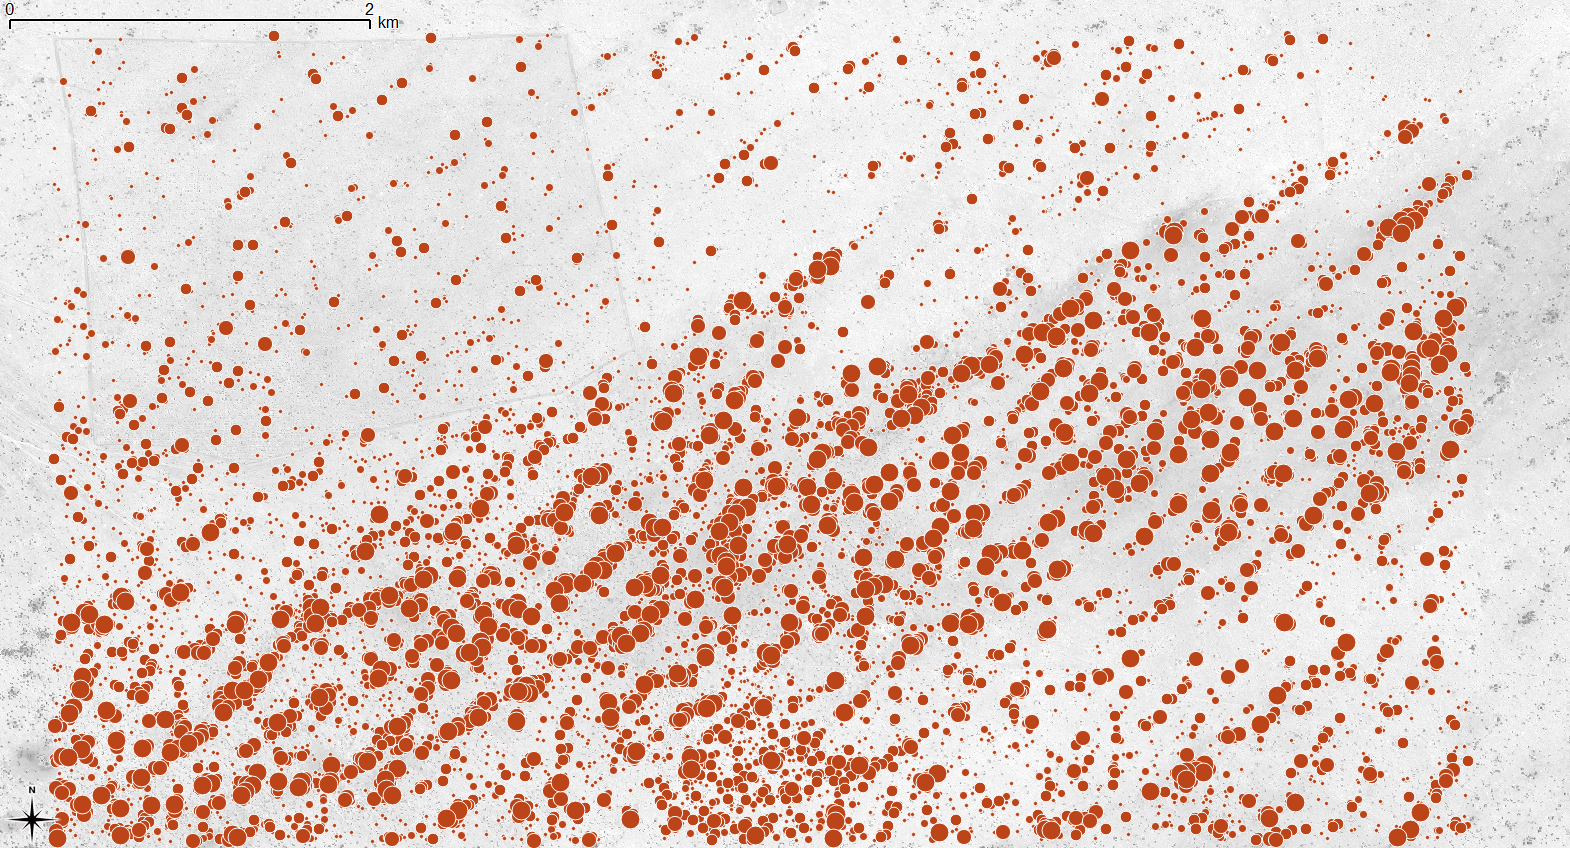
\includegraphics[width = 7cm]{img/Biomasse_arboree}
  \vspace{-1em}
  \caption{Biomass (J.-L.Peiry and D. Ndiaye)}
\end{figure}
\end{frame}

\begin{frame}[c]{WP4 : Resilience and "territorial" management}
\vspace{-2em}
Build a common pool resource management framework for the GGW based on resilience approach and ecosystem services.
\begin{itemize}
  \item Historical analysis for reforestation project
  \item Mapping ecosystem services along the GGW.
  \item Improve the system resilience
\end{itemize}
\begin{figure}
	\centering
	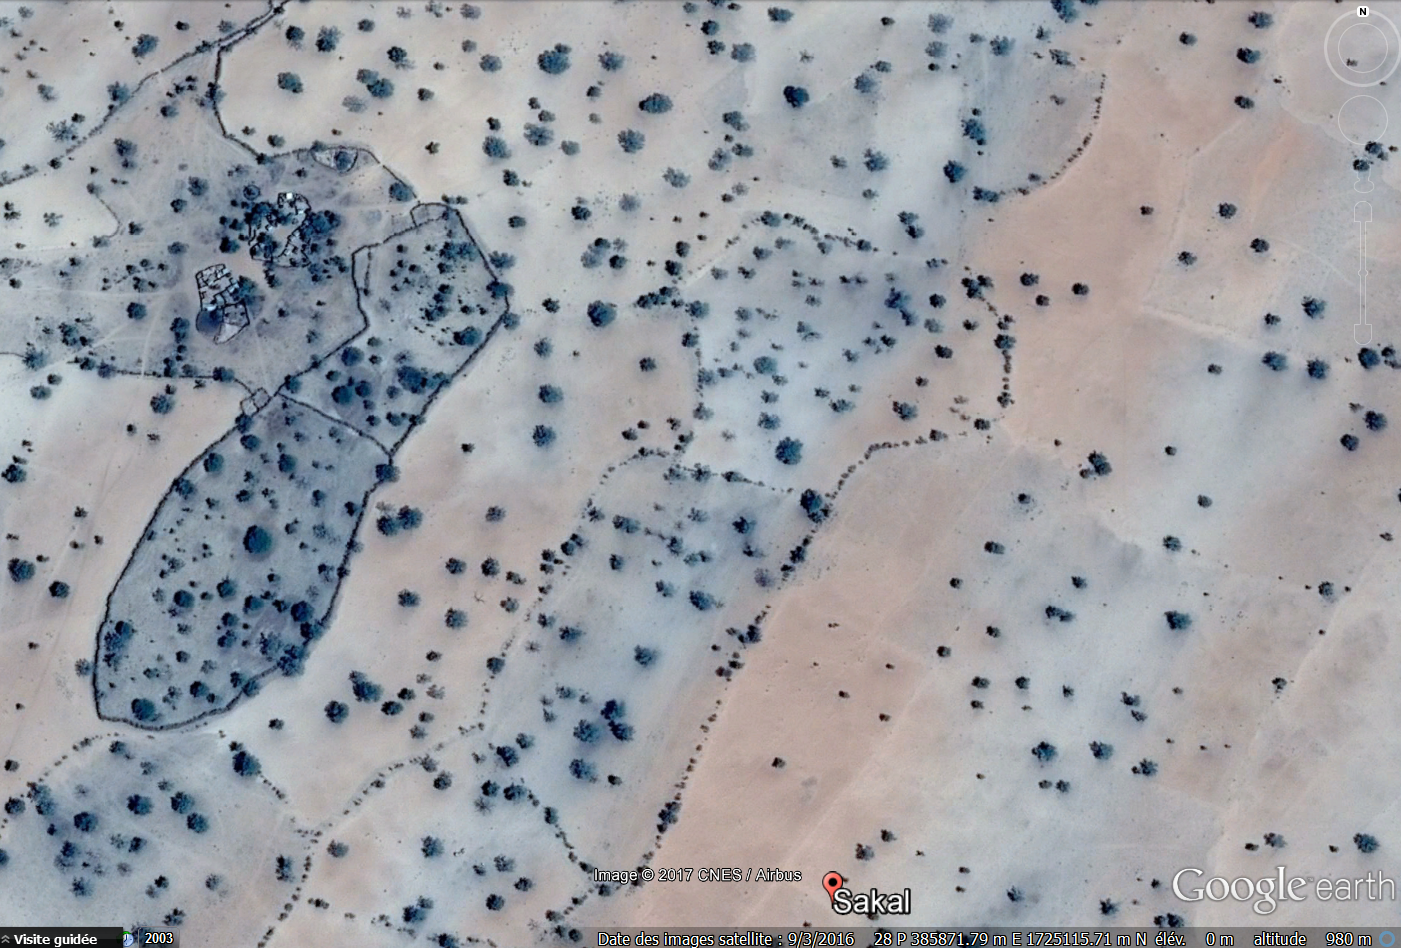
\includegraphics[height = 3.5cm]{img/ggearth}
  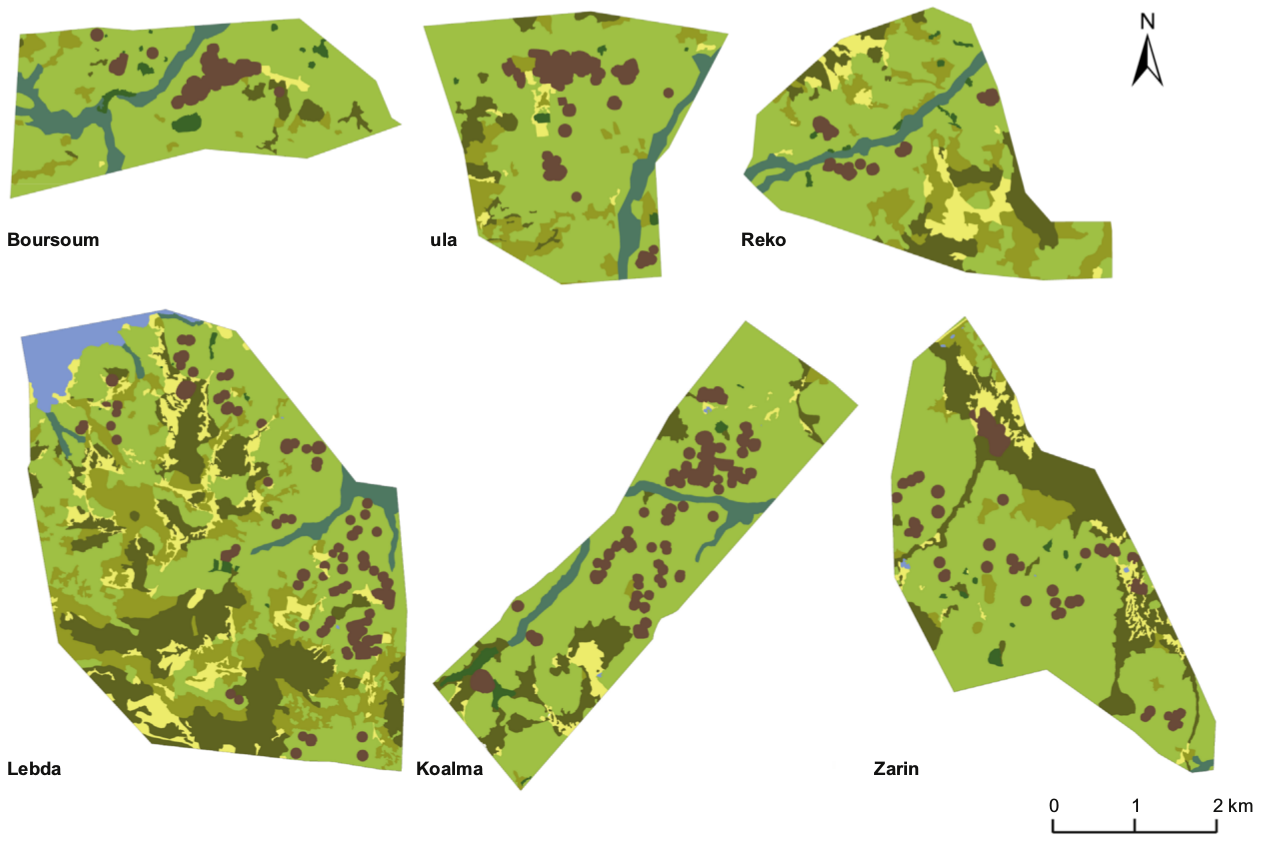
\includegraphics[height = 3.5cm]{img/Sinare_et_al2016}
  \caption{\small{Screenshot Google-earth and maps from Sinare et al. (2016)}}
\end{figure}
\end{frame}

%-=-=-=-=-=-=-=-=-=-=-=-=-=-=-=-=-=-=-=-=-=-=-=-=
%	FRAME: Conclusion
%-=-=-=-=-=-=-=-=-=-=-=-=-=-=-=-=-=-=-=-=-=-=-=-=
\section{Perspective}

\begin{frame}[c]{Post-doctoral research benefit - Agent based modeling and ComMod}
\vspace{-2em}
Create a database is ever the first step of something. My interest is about cooperation and agent-based modeling :
\begin{itemize}
  \item cooperation and emergence
  \item Agent based modeling and ComMod.
\end{itemize}
\begin{figure}
	\centering
	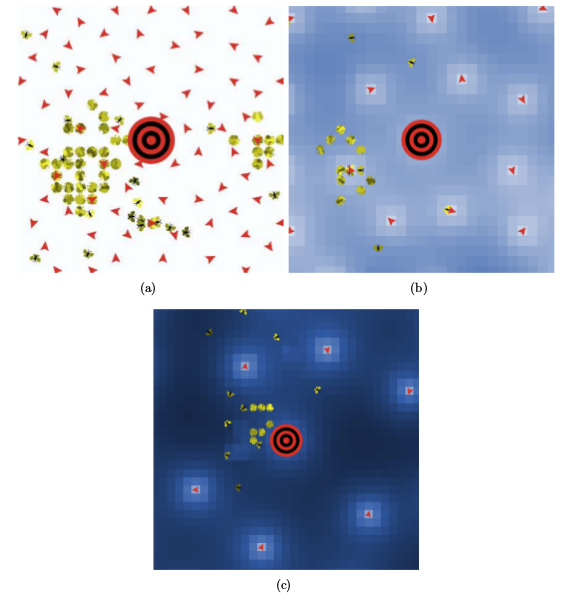
\includegraphics[height = 3.5cm]{img/CeLL_delay2015}
  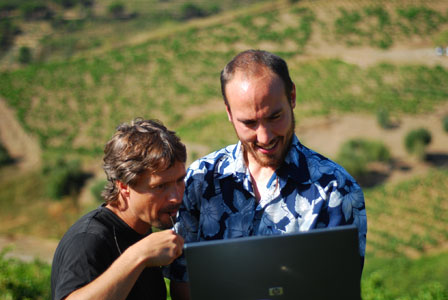
\includegraphics[height = 3.5cm]{img/fielWdelay}
  \caption{\small{CeLL model (Delay 2015)}}
\end{figure}
\end{frame}

\begin{frame}[c]{Post-doctoral research benefit - Cooperation}
\vspace{-2em}
\begin{itemize}
  \item Concept paper proposed in JASSS
  \begin{itemize}
    \item explore irrigation in Mediterranean context
    \item beneficial environmental condition of cooperation emergence
  \end{itemize}
  \item Ferlo is a quiet hard zone for humans. Can we explore this space with our hypothesis in cooperation ?
\end{itemize}
\begin{figure}
	\centering
	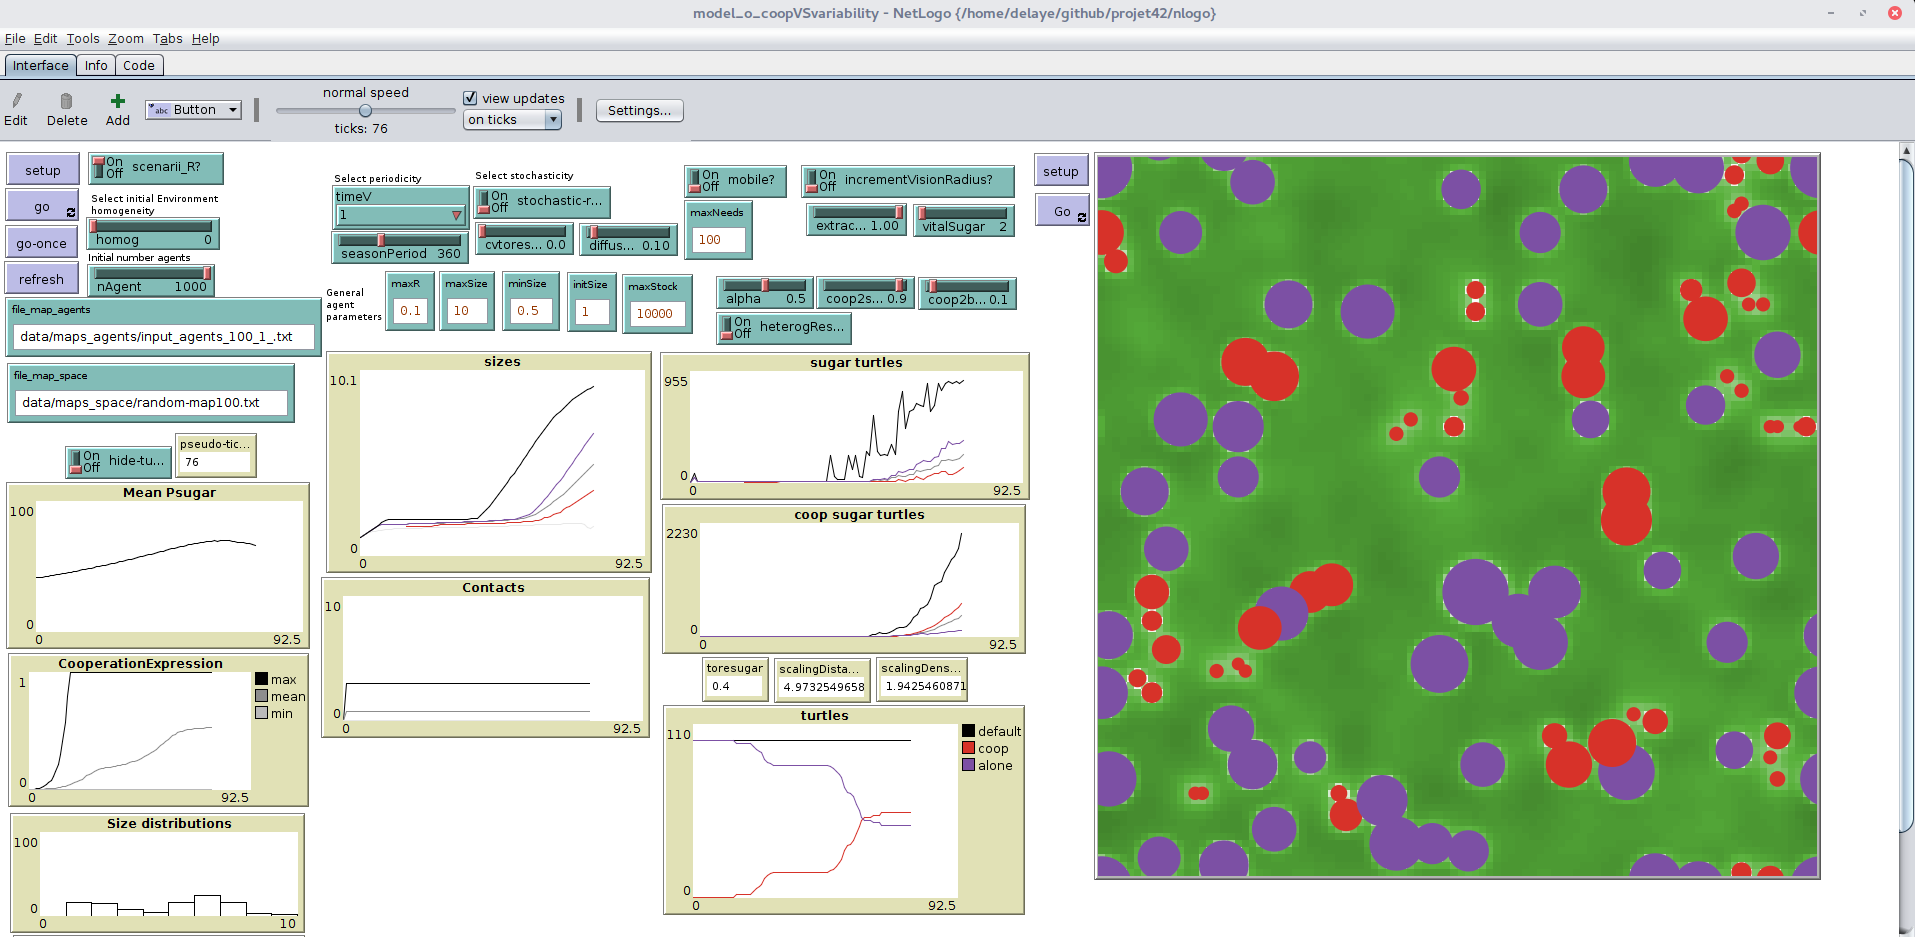
\includegraphics[height = 3.5cm]{img/Proj42}
  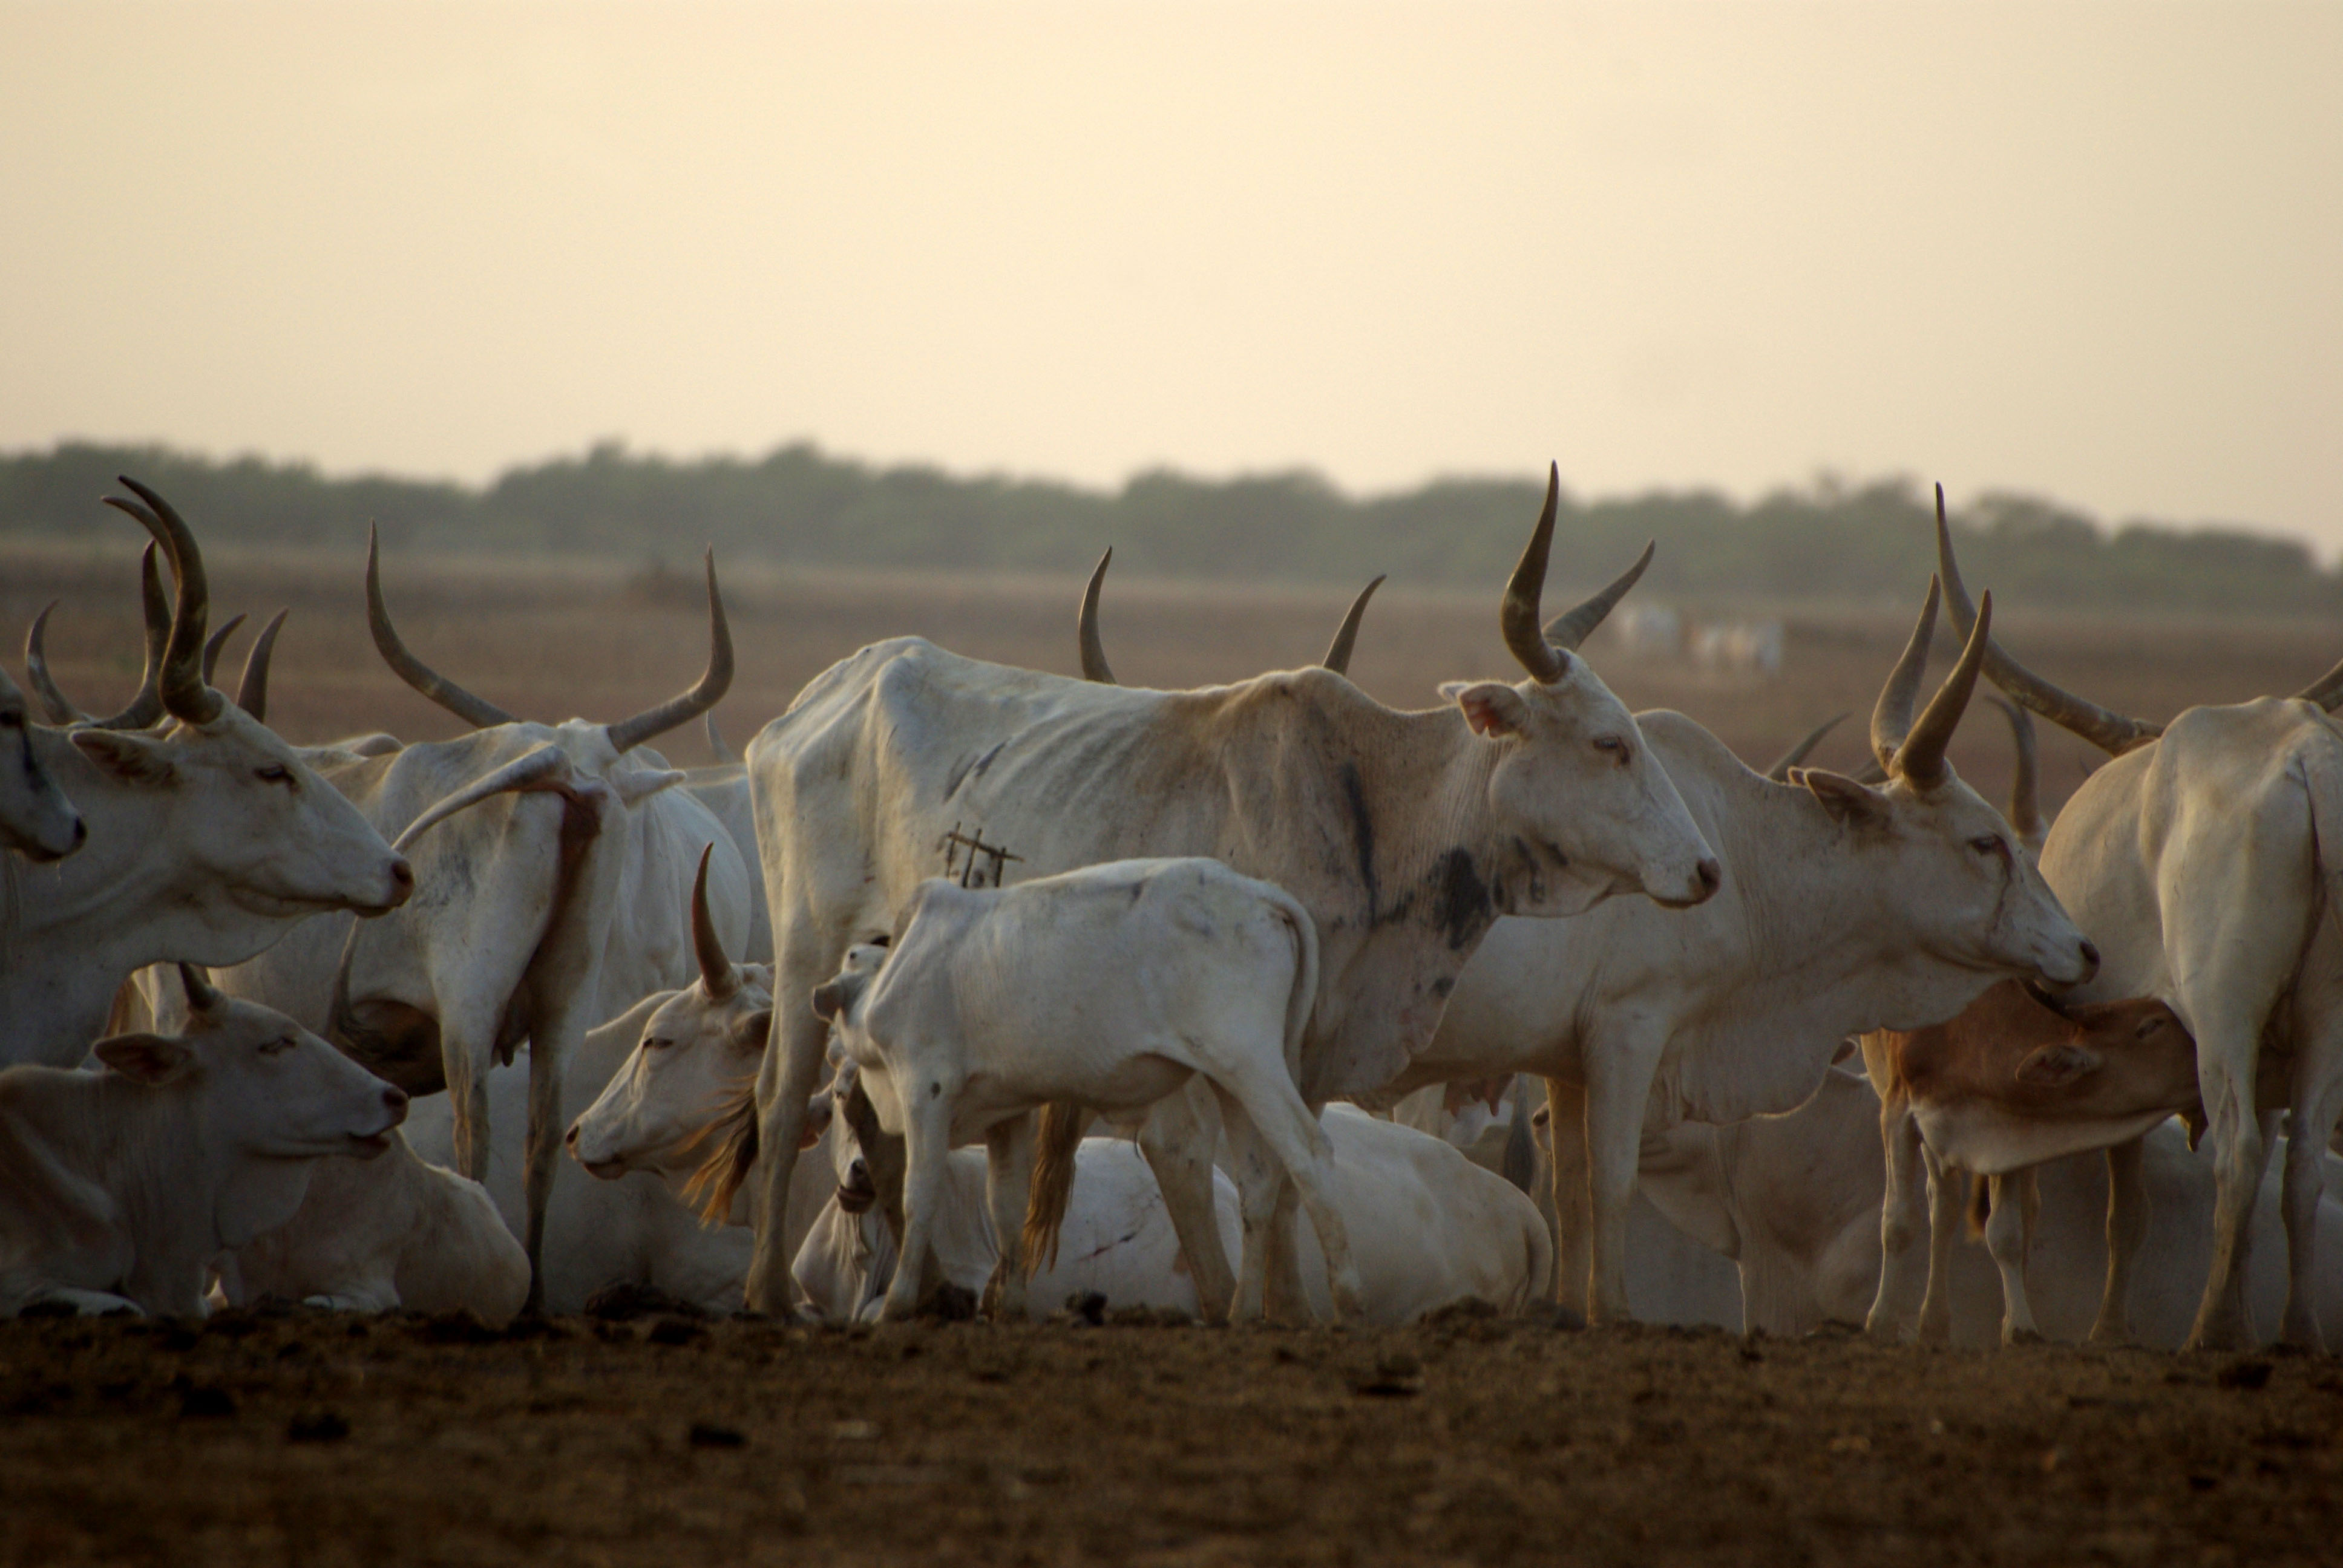
\includegraphics[height = 3.5cm]{img/sng_cow2007}
\end{figure}
\end{frame}
%-=-=-=-=-=-=-=-=-=-=-=-=-=-=-=-=-=-=-=-=-=-=-=-=
%	FRAME: MERCI DE VOTRE ATTENTION
%-=-=-=-=-=-=-=-=-=-=-=-=-=-=-=-=-=-=-=-=-=-=-=-=
{
\usebackgroundtemplate{
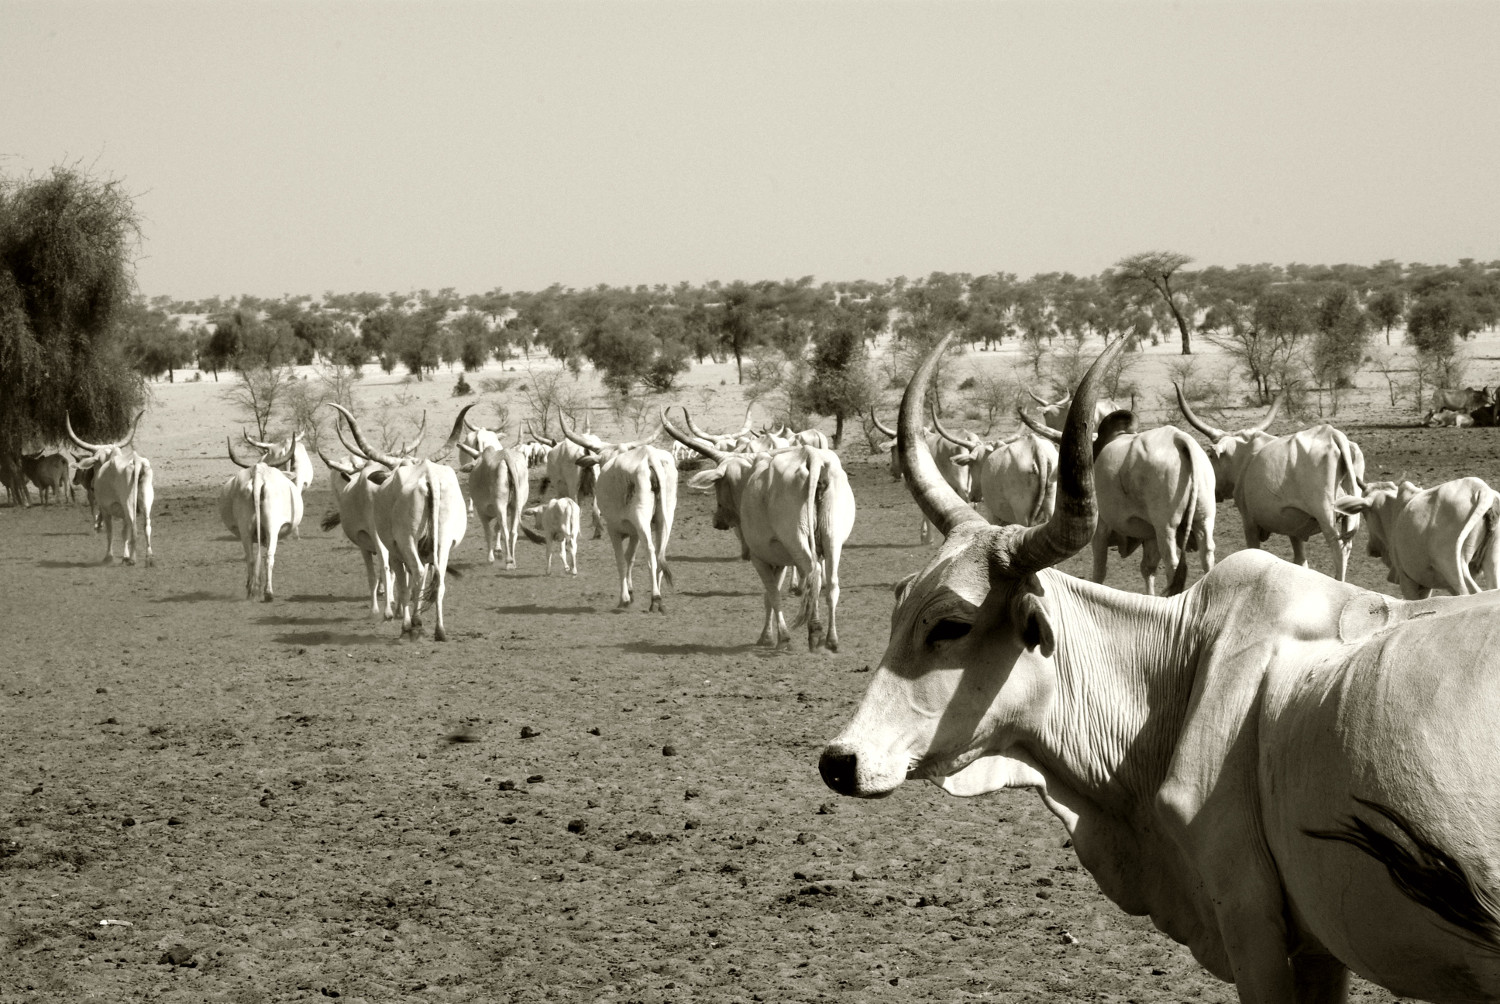
\includegraphics[width=\paperwidth]{img/podor_fin}}%
\begin{frame}
  \vspace{-1em}
  \begin{minipage}[t][.8\textheight]{\textwidth}
    \color{\cnGrey}{\LARGE{Thank you for your attention}}

    \vfill

  %\hfill \small{Photo credit : Thomas m-louis. sur 
\includegraphics[height=0.55cm]{img/flickr_logo}}
  \end{minipage}
  \vspace{-3.5em}
  \centering
	You can find this presentation on github
\includegraphics[height=0.85cm]{img/github}

\end{frame}
}


\end{document}
